\begin{figure}[htbp]
\section*{ TRAF7}
\centering
\begin{subfigure}[b]{0.95\textwidth}
\centering
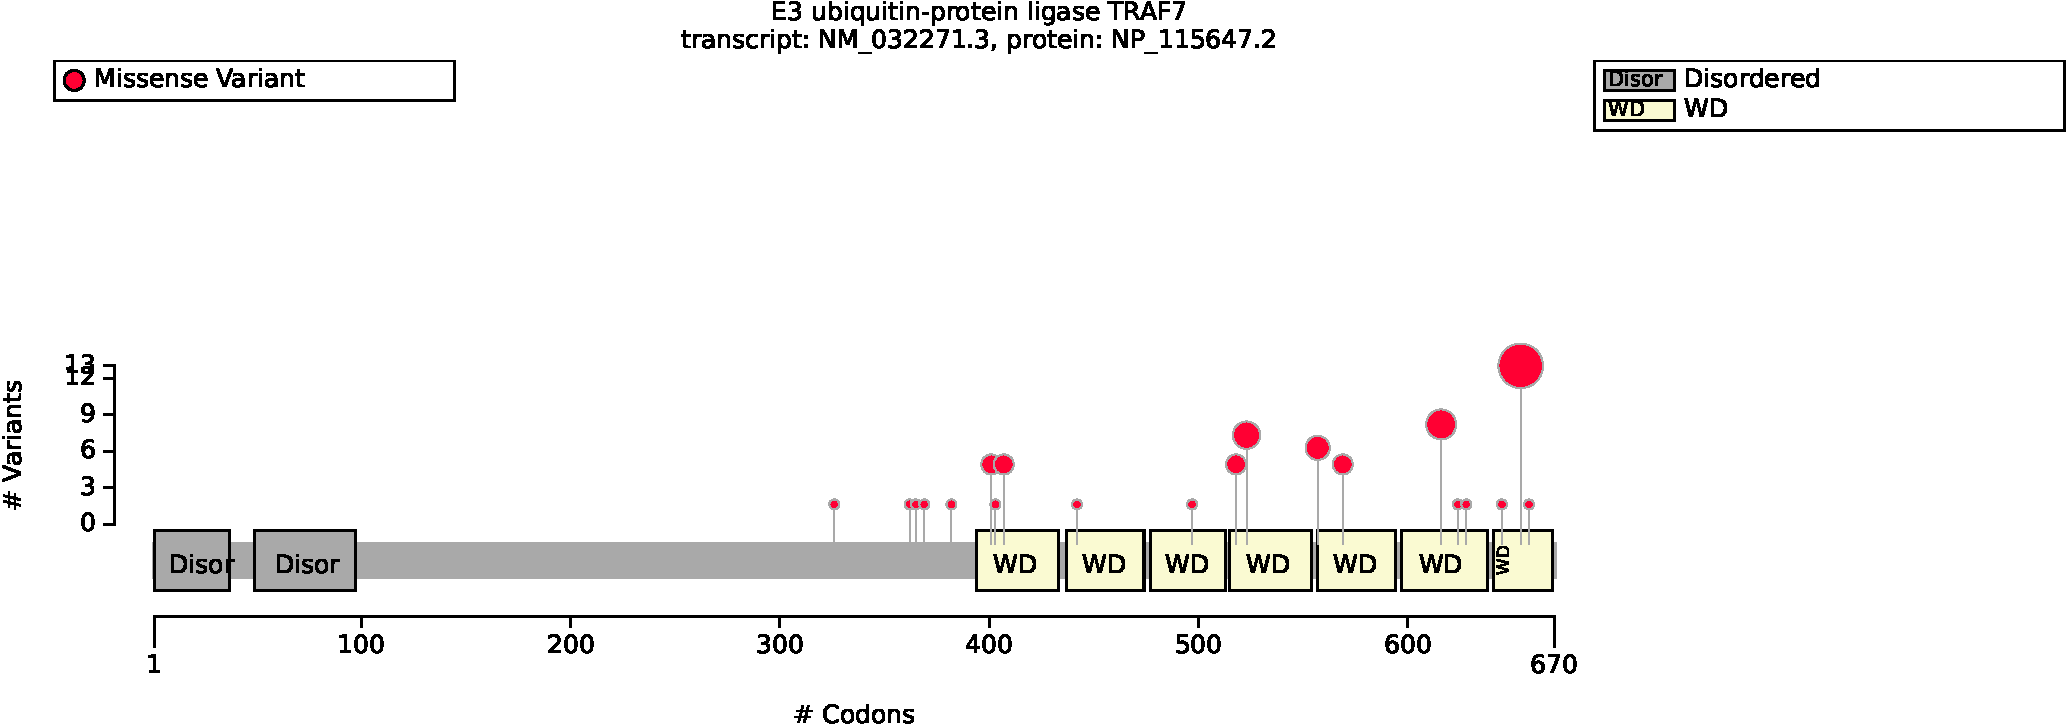
\includegraphics[width=\textwidth]{ img/TRAF7_protein_diagram.pdf} 
\captionsetup{justification=raggedright,singlelinecheck=false}
\caption{Distribution of variants in TRAF7}
\end{subfigure}

\vspace{2em}

\begin{subfigure}[b]{0.95\textwidth}
\centering
\resizebox{\textwidth}{!}{
\begin{tabular}{llllrr}
\toprule
Genotype (A) & Genotype (B) & total tests performed & significant results\\
\midrule
WD7 & other & 40 & 0\\
Arg655Gln & Other variant & 40 & 0\\
FEMALE & MALE & 40 & 0\\
\bottomrule
\end{tabular}
}
\captionsetup{justification=raggedright,singlelinecheck=false}
\caption{Fisher Exact Test performed to compare HPO annotation frequency with respect to genotypes.}
\end{subfigure}

\vspace{2em}

\caption{ The cohort comprised 45 individuals (17 females, 28 males). A total of 360 HPO terms were used to annotate the cohort. Disease diagnosis: Cardiac, facial, and digital anomalies with developmental delay (OMIM:618164). No significant correlations identified. A total of 23 unique variant alleles were found in \textit{TRAF7} (transcript: \texttt{NM\_032271.3}, protein id: \texttt{NP\_115647.2}).}
\end{figure}
